% Codata assignment 2-pager — LaTeX template.
% Build: pdflatex main.tex  (or latexmk -pdf main.tex)
\documentclass[10pt,a4paper]{article}

\usepackage[margin=1.9cm]{geometry}
\usepackage[T1]{fontenc}
\usepackage[utf8]{inputenc}
\usepackage{helvet}\renewcommand{\familydefault}{\sfdefault}
\usepackage{graphicx}
\usepackage{booktabs}
\usepackage{enumitem}
\usepackage[hidelinks]{hyperref}
\usepackage{titlesec}

% compact spacing for the 2-page limit
\titleformat*{\section}{\normalsize\bfseries}
\titlespacing*{\section}{0pt}{6pt}{3pt}
\setlist[itemize]{leftmargin=1.2em, itemsep=1pt, topsep=2pt, parsep=0pt}
\setlength{\parindent}{0pt}
\setlength{\parskip}{2pt}

\title{\vspace{-1.4cm}\large\bfseries Text-to-Wikidata Entity Linking: a GraphRAG-inspired Pipeline}
\author{}
\date{}

\begin{document}
\maketitle
\vspace{-1.6cm}

\textbf{Goal:} a lightweight Python pipeline that identifies meaningful terms (not only named entities) in unstructured text and links each to the right Wikidata concept. 

\textbf{Hypothesis:} graph context from Wikidata improves the entity-linking (disambiguation) step. The pipeline runs fully locally (spaCy + small Ollama models), and every design decision below was made based on the experiments done on the candidate generator and the ranker; the resulting architecture is shown in Fig.~\ref{fig:arch}. \emph{The appendix and references are outside the 2-page limit.}

\textbf{Dataset:} built from ELEVANT~\cite{elevant} (EMNLP 2022, Uni Freiburg), chosen because it annotates entities beyond named entities. Gold QIDs were re-validated against current Wikidata, and the set was stratified into ambiguous vs non-ambiguous mentions, crossed with the NER outcome of step~1 (ambiguous/non-ambiguous $\times$ ner/no-ner). Documents were sampled by taking those with the most mentions, keeping all mentions of a chosen document and breaking ties to keep the ambiguity split closest to even.

\section*{1. Text processing and term extraction}
\begin{itemize}
  \item spaCy (small model) splits paragraphs into sentences and extracts POS, noun phrases, lemmas and named entities. Each mention is expanded with its lemma, stem and WordNet synonyms for retrieval.
  \item \textbf{Decision 1 --- spaCy alone misses non-named-entity mentions.} Instead of a large NER model, d1-omni:600m answers typed NER questions with a calibrated probability per option in one forward pass. The decision model is a 600\,M-parameter encoder served locally via the Ollama model library~\cite{d1omni}. Merging spaCy with the decision model raised mention coverage:
\end{itemize}

\begin{center}\small
\begin{tabular}{@{}lc@{}}
\toprule
Term extraction & Mention coverage \\
\midrule
spaCy (small) alone & 61/94 $\approx$ 65\% \\
spaCy + d1-omni:600m & \textbf{90/100 = 90\%} \\
\bottomrule
\end{tabular}
\end{center}

\section*{2. Candidate retrieval (Wikidata API)}
\begin{itemize}
  \item Each mention form (surface, lemma, stem, synonyms) is queried in parallel; candidates are cached in a SQLite store with QID, label, description, aliases and 1-hop triples. For graph context, each candidate's 1-hop triples are fetched from Wikidata already at this stage. The stage is tuned for recall; selection is left to the ranker.
  \item \textbf{Decision 2 --- wbsearchentities over CirrusSearch.} Cirrus full-text search surfaces less prominent entities that merely contain the query words; wbsearchentities ranks by prominence, which matches how mentions are used in text. The Cirrus recall drop is the negative result behind this decision:
\end{itemize}

\begin{center}\small
\begin{tabular}{@{}lccc@{}}
\toprule
Candidate retrieval & Overall recall & Ambiguous & Non-ambiguous \\
\midrule
wbsearchentities & \textbf{68/90 = 75.6\%} & 27/44 = 61.4\% & 41/46 = 89.1\% \\
CirrusSearch (full-text) & 35/90 = 38.9\% & 19/44 = 43.2\% & 16/46 = 34.8\% \\
\bottomrule
\end{tabular}
\end{center}

\begin{itemize}
  \item \textbf{Insight.} Candidate recall is the ceiling on end-to-end accuracy, and the misses concentrate on ambiguous mentions (61.4\% vs 89.1\%) --- on those, the generator, not the ranker, is the bottleneck. Recall-oriented query expansion (lemma, stem, synonyms) plus prominence-ranked search hold overall recall at 75.6\%.
\end{itemize}

\section*{3. Knowledge graph enrichment}
\begin{itemize}
  \item For every candidate, its Wikidata triples are fetched and stored. Per document, a NetworkX graph connects all candidates of all mentions: nodes are QIDs, edges are Wikidata properties, both keeping their RDF terms (wd:/wdt: IRIs), following the RDF/SKOS framing.
  \item This graph is the disambiguation signal: correct candidates pull together into a connected cluster --- e.g.\ Belarus, Germany and Ireland link via ``diplomatic relation'' --- while wrong candidates (the element germanium, the person Samuel Ireland) stay isolated (Fig.~\ref{fig:graph}).
\end{itemize}

\section*{4. GraphRAG-based candidate selection --- ranker architecture and experiments}
\emph{Note on the GraphRAG framing: a RAG pipeline usually retrieves from a dedicated vector or graph database; here Wikidata itself is the graph database, and retrieval from it happens at the candidate-generation phase (steps 2--3).}

\textbf{Base scorer (all variants):} cosine similarity between the embedding of ``mention + sentence'' and each candidate rendered as ``label: description (aliases)'' (embeddinggemma), plus small lexical priors: Wikidata's own search rank (0.15/rank), exact label match (+0.10) and a Levenshtein penalty ($-$0.05). GraphRAG enters in two ways:
\begin{itemize}
  \item \textbf{Retrieval-augmentation:} each candidate's graph neighbourhood is verbalised into up to 12 facts and appended to the candidate text before embedding.
  \item \textbf{Graph coherence bonus (weight 0.2):} a candidate directly connected to another mention's candidate scores 1.0, a shared neighbour 0.5, an isolated candidate 0.
\end{itemize}

Seven ranker variants (cr\_v1--v7) were built on this scorer and compared on the full stratified run:

\begin{center}\footnotesize
\renewcommand{\arraystretch}{0.95}
\begin{tabular}{@{}lcccr@{}}
\toprule
Ranker (full stratified run) & Overall acc/MRR & Ambiguous & Non-ambiguous & Time \\
\midrule
v1 embed (embeddinggemma) & 57.8\% / 0.64 & 40.9\% / 0.48 & 73.9\% / 0.79 & 14 s \\
v2 embed + graph          & \textbf{63.3\% / 0.67} & \textbf{47.7\% / 0.52} & \textbf{78.3\% / 0.82} & 19 s \\
v3 d1 (d1-omni:600m)      & 62.2\% / 0.67 & 45.5\% / 0.52 & \textbf{78.3\% / 0.82} & 15 s \\
v4 d1 + graph             & 60.0\% / 0.66 & 45.5\% / 0.52 & 73.9\% / 0.79 & 14 s \\
v5 AMR graph (amrlib)     & 60.0\% / 0.64 & 47.7\% / 0.51 & 71.7\% / 0.76 & 858 s \\
v6 AMR + d1               & 56.7\% / 0.63 & 38.6\% / 0.47 & 73.9\% / 0.79 & 28 s \\
v7 graph-embed (NetMF-style) & 57.8\% / 0.64 & 38.6\% / 0.47 & 76.1\% / 0.80 & 19 s \\
\bottomrule
\end{tabular}
\end{center}

\textbf{Decisions made from these experiments:}
\begin{itemize}
  \item \textbf{Embedding vs decision-model ranking.} v3/v4 phrase ranking as one d1 choice question (candidates as options, calibrated probability per candidate as the score). The d1 rankers land just behind the embeddings (62.2\% / 60.0\% vs 63.3\%), but graph context only helps the embedding family (v1$\to$v2, +5.5 points overall); for d1 it slightly hurts (v3$\to$v4, $-$2.2) --- the verbalised facts lengthen the options without adding discriminative evidence for the decision model.
  \item \textbf{Verbalised vs structural graph embeddings.} v7 replaces the verbalised facts with structural node embeddings (NetMF-style) and scores by cosine to the centroid of the other mentions' candidate vectors. It matched the no-graph baseline overall (57.8\%) but lost to verbalised graph context on ambiguous mentions (38.6\% vs 47.7\%).
  \item \textbf{Negative results --- AMR graphs (v5/v6).} v5 parses each sentence into an AMR graph (amrlib) and matches graph-to-graph; it ties v2 on ambiguous mentions (47.7\%) but trails overall (60.0\% vs 63.3\%) and takes 858~s --- $\sim$45$\times$ slower --- ruling it out. v6 feeds the same AMR facts into a d1 choice question and drops to 56.7\% overall, joint-worst on ambiguous mentions (38.6\%, with v7): stacking verbalised graphs on both sides dilutes the evidence instead of sharpening it.
  \item \textbf{Final ranker: v2 (embeddings + verbalised graph facts + coherence bonus).} Graph context lifts overall accuracy 57.8\% $\to$ 63.3\% and ambiguous accuracy 40.9\% $\to$ 47.7\% over the no-graph baseline. The top candidate is returned only when evidence is sufficient, otherwise alternatives are surfaced.
  \item \textbf{Insight.} Graph context gives its gain exactly where disambiguation is hardest --- ambiguous mentions (+6.8 points, v1$\to$v2) --- but only when paired with the embedding ranker. How the graph is used matters more than the ranking model: verbalised facts beat both structural embeddings (v7) and AMR graphs (v5/v6). MRR above accuracy (0.67 vs 63.3\%) means that when rank~1 is wrong the gold entity is usually just below it, so the surfaced alternatives often contain the right answer.
\end{itemize}

\section*{5. Output and evaluation}
\begin{itemize}
  \item Output is structured JSON per mention: original term and sentence, selected concept with QID, rank, score, confidence and supporting evidence, plus the ranked alternative candidates.
  \item Evaluation compares the no-graph baseline against the graph-context ranker on the stratified set (table above): the graph context gives the largest gain exactly where disambiguation is hardest, confirming the hypothesis.
\end{itemize}

\section*{6. Future work}
\begin{itemize}
  \item The ranker can be experimented with different language models: other embedding and decision models drop into the same base scorer.
  \item Different graph embeddings can be applied in place of NetMF --- e.g.\ translational models such as TransE over the candidate graphs.
  \item For GraphRAG, a local graph database (e.g.\ FalkorDB) can be set up: 1--4-hop triples fetched from Wikidata and stored in the graph database (or a vector database), then queried at the ranker phase --- more precise graph information than the current 1-hop candidate store.
  \item More work on the AMR front (v5): the sentence itself is converted into a graph, and graph-to-graph matching happens at the ranking phase --- promising on ambiguous mentions, but it needs a faster parser.
\end{itemize}

{\footnotesize
\textbf{Code and experiments:} \url{https://github.com/itisha2/text-to-wikidata-linking} (main branch) --- \texttt{src/} holds the text-preprocessing, candidate-generator and ranker code; \texttt{src/ranker/} has all seven ranker experiments (\texttt{cr\_v1}--\texttt{cr\_v7}). \texttt{inference\_pipeline.ipynb} implements the final entity-linking pipeline by importing these modules and can be run against any text or paragraph; candidate retrieval may take a while, as its latency depends on the Wikidata search API.

\textbf{AI usage declaration.} AI assistance was used for code polishing and for paraphrasing the write-up. The dataset selection, the candidate-generator and ranker experiment design, the decision and evaluation criteria, and the baseline code implementation are the author's own.
}

\newpage
\section*{Appendix}
\begin{figure}[h]
\centering
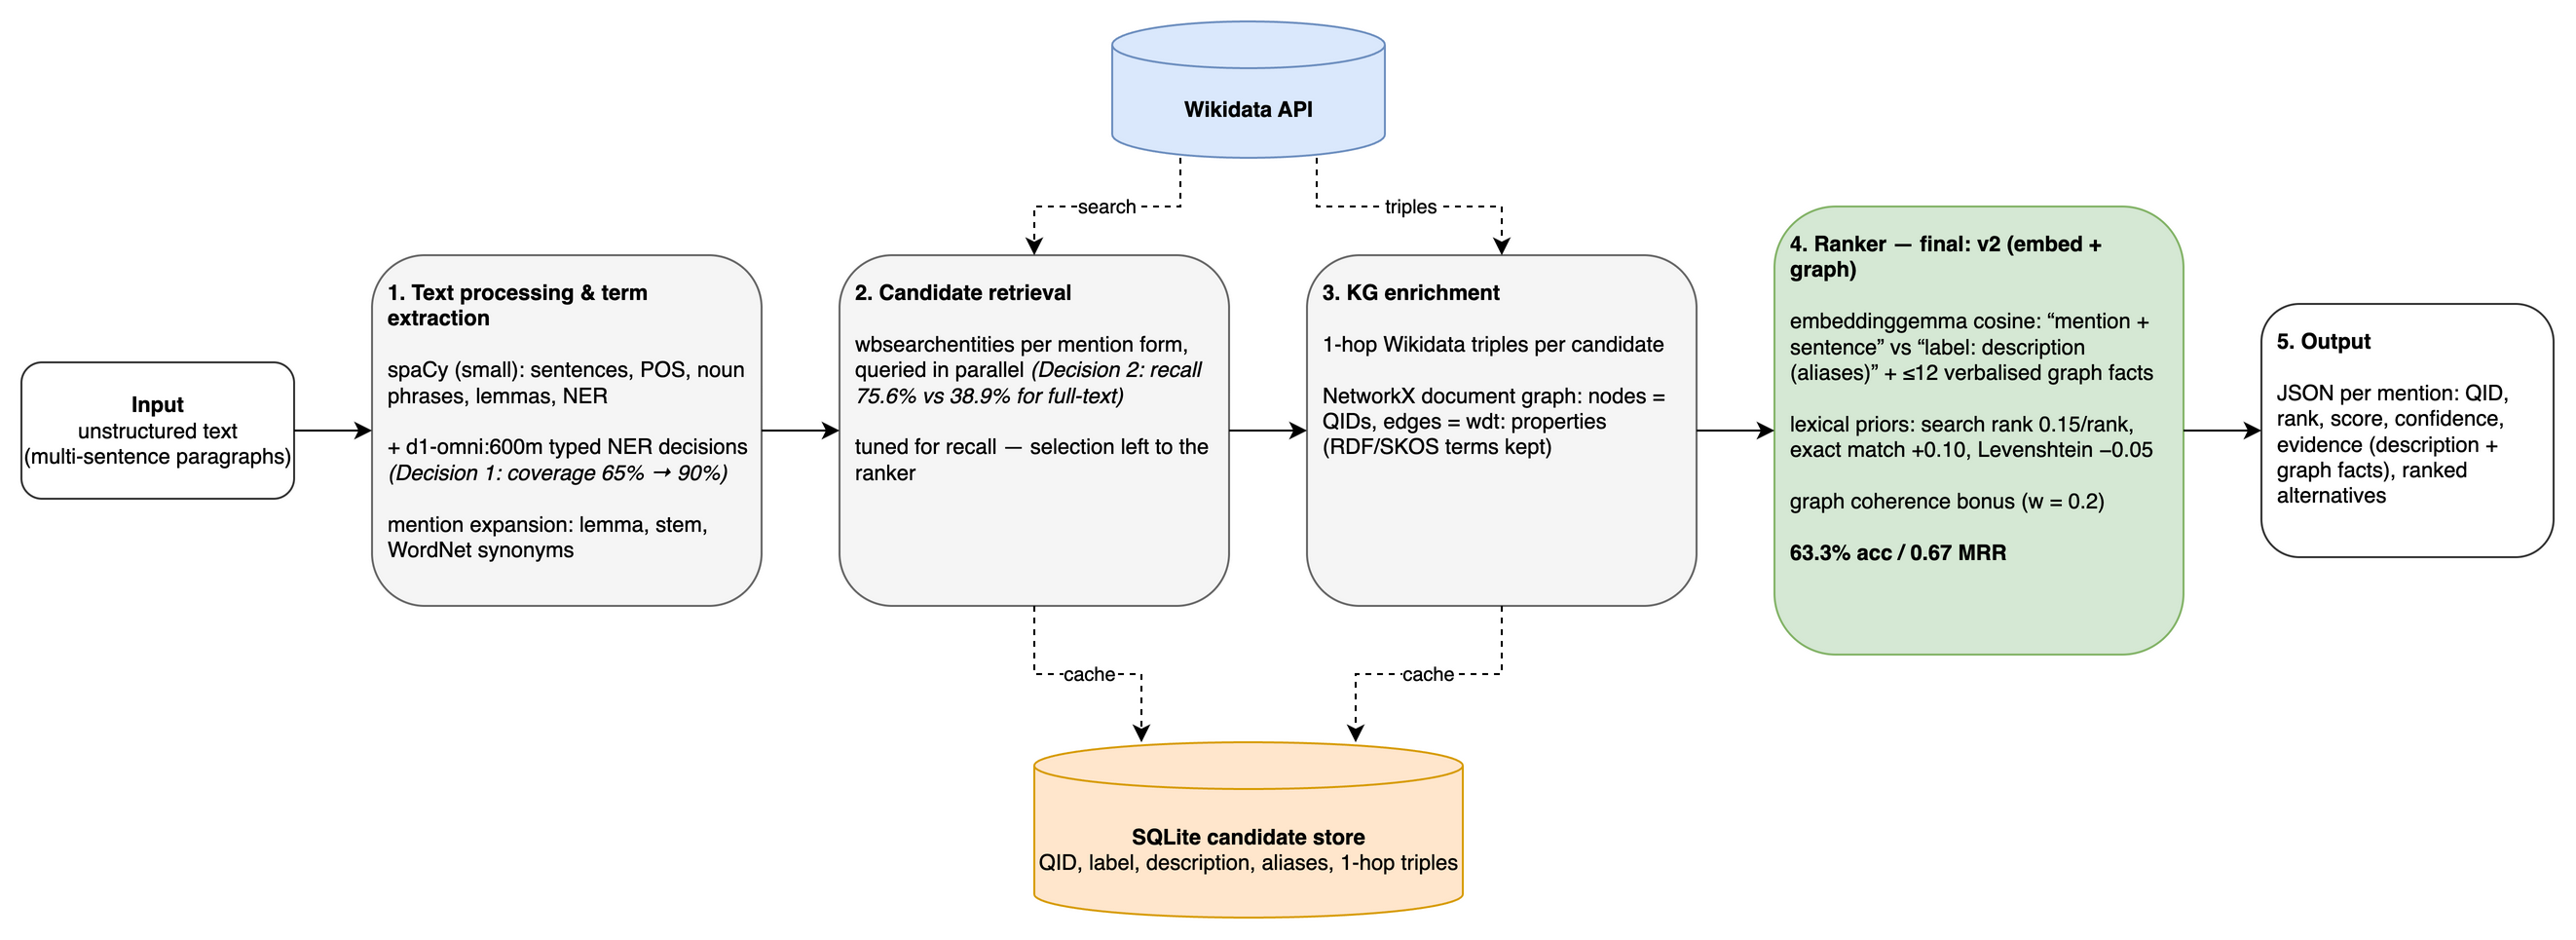
\includegraphics[width=\textwidth]{architecture.png}
\caption{Final pipeline architecture after Decisions 1--2 and the ranker experiments (final ranker: v2).}
\label{fig:arch}
\end{figure}

\begin{figure}[h]
\centering
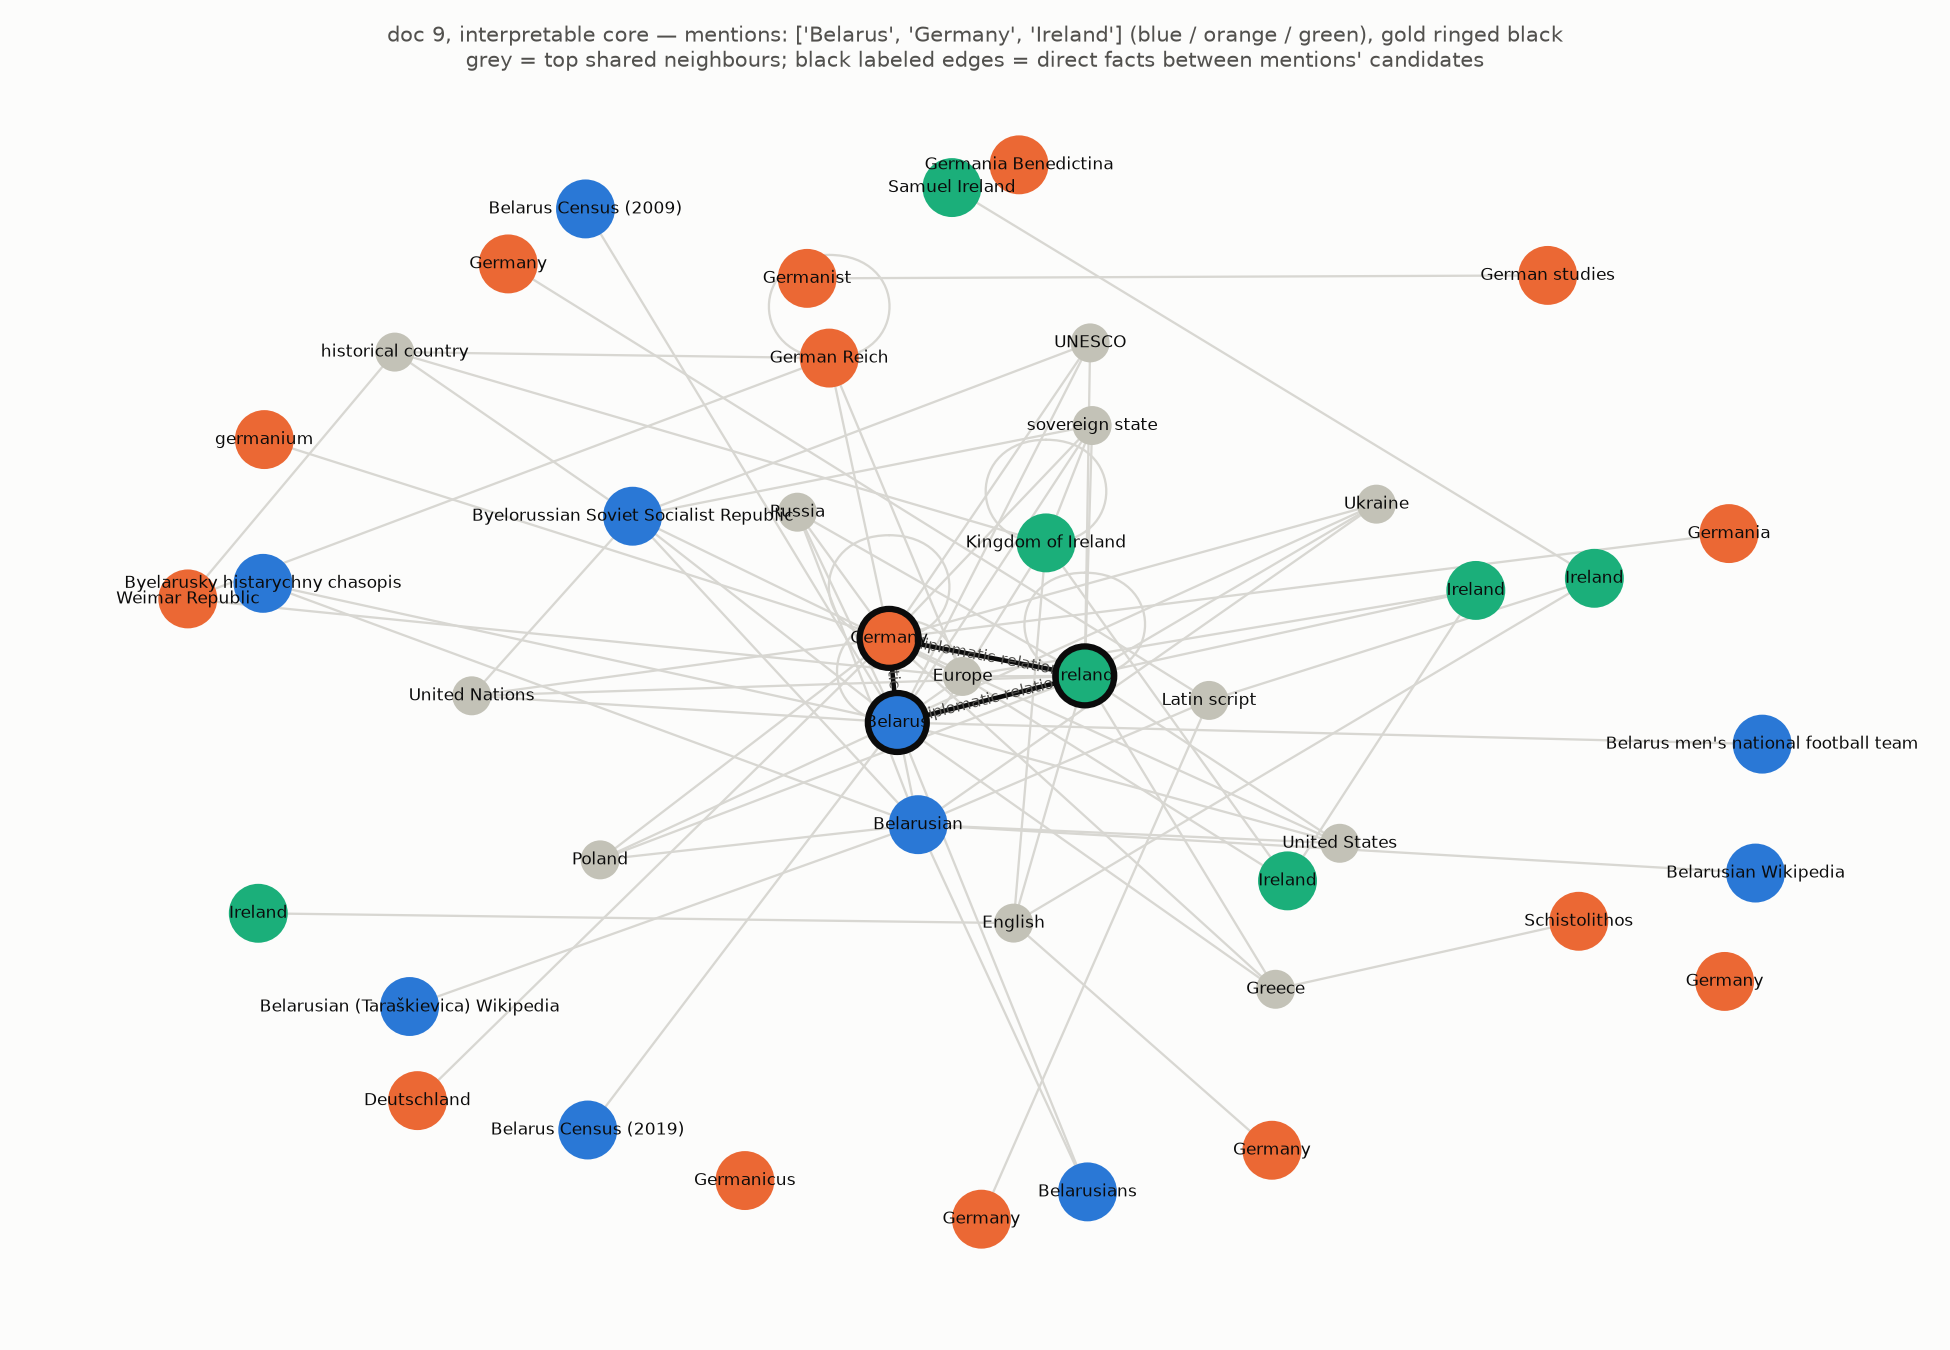
\includegraphics[width=0.85\textwidth]{doc9_graph_core.png}
\caption{Document-level candidate graph (document 9). The correct candidates (Belarus, Germany, Ireland) form a tightly connected core via ``diplomatic relation'' edges, while wrong candidates with the same surface forms (the chemical element germanium, the person Samuel Ireland) have no connections to the rest of the document and drift to the periphery. The coherence bonus scores exactly this structure.}
\label{fig:graph}
\end{figure}

\begin{thebibliography}{2}
\bibitem{elevant} Hannah Bast, Matthias Hertel, Natalie Prange. 2022. ELEVANT: A Fully Automatic Fine-Grained Entity Linking Evaluation and Analysis Tool. In \emph{Proceedings of EMNLP 2022: System Demonstrations}. \url{https://aclanthology.org/2022.emnlp-demos.8/}
\bibitem{d1omni} d1-omni:600m decision model. Ollama model library. \url{https://ollama.com/library/d1-omni:600m}
\end{thebibliography}

\end{document}
